\chapter{Pruebas de Hipótesis}

% []
% \tableofcontents
% 

\paragraph{Conceptos Estadísticos Importantes}
 \begin{enumerate}
  \item Pruebas de hipótesis.
  \item $p-$valores.
  \item Distribución normal.
  %\item Correlación.
 \end{enumerate}


\paragraph{Muestreo aleatorio y teorema del límite central}
 Entender el concepto de \emph{muestreo aleatorio} a través de ejemplos e ilustrar las aplicaciones del \emph{teorema del límite central}. 

%  Estos dos conceptos son la columna vertebral de las pruebas de hipótesis.


\paragraph{Pruebas de hipótesis}
 Entender el significado de los términos tales como \emph{hipótesis nula}, \emph{hipótesis alternativa}, \emph{intervalos de confianza}, \emph{$p-$valores}, \emph{nivel de significación}, etc.
%   Desarrollaremos una guía de la implementación de pruebas de hipótesis, seguidas por un ejemplo.

\paragraph{Pruebas $\chi-$cuadrada}
 Calcularemos el estadístico $\chi$-cuadrada y describiremos el uso de pruebas $\chi$-cuadrada con un par de ejemplos.

% \paragraph{Correlación}
%  Entenderemos el significado y la significación de la correlación entre dos variables, de los coeficientes de correlación y calcularemos y visualizaremos la correlación entre variables de una base de datos.
% 

\section{Muestreo aleatorio y teorema del límite central}

\paragraph{Ejemplo}
 Supongamos que tratamos de encontrar la edad promedio en una ciudad, digamos Oaxaca. Una manera de hacerlo sería por \emph{fuerza bruta}, es decir, recolectando esta información persona por persona. Pero este método sería muy costoso en términos de infraestructura y tiempo.


 En estadística, este es un problemalema común, cuya solución está en el \emph{muestreo aleatorio}:  Tomemos un grupo de 1000 individuos (o 10,000 dependiendo de tu capacidad, obviamente entre más, es mejor) y calculemos la edad promedio en este grupo, a la que denotaremos por $A_{1}.$ 


 Repitamos este procedimiento, digamos 100 veces, y denotaremos por $A_{1}, A_{2},...,A_{100}$ el promedio de edades obtenido en cada respectivo intento.
 
 De acuerdo a la \emph{ley de los grandes números}, la cantidad
 \begin{align}
  \bar{A}_{100}=\dfrac{A_{1}+...+A_{100}}{100}
 \end{align}
es una aproximación muy cercana al promedio real de la edad de los pobladores de la ciudad.


 De acuerdo al \emph{teorema del límite central}, si el número de tales muestras es suficientemente grande,
 $A_{1},A_{2},...,A_{100}$ estarán distribuidos de manera normal.


 \begin{rem}
  No estamos más interesados en obtener el valor exacto de la edad promedio, si no establecer un \emph{estimador} para la misma. 

  En tal caso,
tenemos que conformarnos con la definición de un \emph{rango de valores} en el que el valor real podría estar.
 \end{rem}


% 
% Dado que hemos supuesto una \emph{distribución normal} para los valores de edad media de estos
% grupos, podemos \emph{aplicar todas las propiedades} de una distribución normal para
% posibilidades de que la edad \emph{promedio} este en algún \emph{intervalo}.
% 

\section{Pruebas de hipótesis}
% 
% El concepto que acabamos de comentar en la sección anterior se utiliza para una
% técnica en estadística, llamada \emph{prueba de hipótesis}.
% 


En la prueba de hipótesis, asumimos una
premisa inicial (generalmente relacionada con el valor del estimador) denominada \emph{hipótesis nula}  y
trataremos de ver si es cierta o no aplicando.



Tenemos otra premisa llamada \emph{hipótesis alternativa}, la cuál es la negación de la hipótesis nula.


\paragraph{Hipótesis nula vs. alternativa}
%  Hay una forma para decidir cuál será la hipótesis nula y cuál será la hipótesis alternativa. 
%
% La hipótesis nula es la premisa inicial o algo que
% podemos suponer que es cierto. 
%
% Por el contrario, la hipótesis alternativa es algo de lo que no estamos seguros que podría ser cierto.
% 
%
% 
 Cuando alguien está haciendo una \emph{investigación} cuantitativa para calibrar el valor de un estimador,  el \emph{valor conocido} del parámetro se toma como \emph{hipótesis nula},  mientras que el \emph{nuevo valor} encontrado (de la investigación) se toma como la \emph{hipótesis alternativa}.
 


 En nuestro caso (encontrar la edad media de nuestra ciudad), un investigador puede afirmar que la edad
\emph{menor que 35}. Esto puede servir como la \emph{hipótesis nula}.


Si una nueva agencia afirma
que es \emph{mayor que 35}, entonces se puede denominar como la \emph{hipótesis alternativa}.


\section{Estadísticos Z y t}

\begin{enumerate}
 \item Suponga que el valor del parámetro asumido en la hipótesis nula es $Ao$. 
 \item Tomemos
una muestra aleatoria de 100 o 1000 personas o eventos del evento. 
\item Calculemos
la media del parámetro, por ejemplo la edad promedio de una ciudad, el tiempo medio de suministro de la pizza, la media
ingresos, etc. 
\item Podemos llamarlo $A$.
\end{enumerate}




El estadístico $Z$ se calcula para convertir una variable normalmente distribuida (por ejemplo, la distribución de la media poblacional de edad) a una distribución normal estándar.
%  Esto es porque los valores de problemaabilidad para una variable que sigue a la distribución normal estandarizada se puede obtener de una tabla precalculada.


El estadístico $Z$ se da por la siguiente fórmula:
\begin{align}
 \label{zStat}
 Z=\dfrac{A-A_{0}}{{\sigma}/{\sqrt{n}}}
\end{align}
donde $\s$ es la desviación estándar de la población y $n$ es el número de personas en la muestra


Ahora, debemos considerar dos casos

\paragraph{Prueba Z (distribución normal)}
El investigador conoce a desviación estándar del parámetro de su experiencia pasada.



Un buen ejemplo de esto es el caso del tiempo de entrega de una pizza.  En este caso \eqref{zStat} seguirá una distribución normal y los valores normalizados se conocerán como \emph{valores Z}.

\paragraph{Prueba t (distribución t de Student) }
En este caso, el investigador no conoce la desviación estándar de la población.



Esto puede pasar porque:
\begin{itemize}
 \item No existen tales datos en algún registro histórico;
 \item o el número de eventos o personas es demasiado pequeño para suponer una distribución normal.
\end{itemize}


En este caso, la media y la desviación estándar son desconocidas, y la expresión asume una distribución diferente a la normal llamada \emph{distribución $t$ de Student}.



El valor estandarizadas en este caso es llamado \emph{$t-$valor} y la prueba es llamada \emph{prueba-$t$}.


\paragraph{Distribución t de Student}
\begin{quote}
 La distribución de Student fue descrita en 1908 por William Sealy Gosset. Gosset trabajaba en una fábrica de cerveza, Guinness, que prohibía a sus empleados la publicación de artículos científicos debido a una difusión previa de secretos industriales. De ahí que Gosset publicase sus resultados bajo el seudónimo de Student. \footnote{
\href{https://es.wikipedia.org/wiki/Distribuci\%C3\%B3n\_t\_de\_Student\#Historia}{Wikipedia: Distribución $t$ de Student}
}
\end{quote}


\begin{figure}[h]
 \centering
 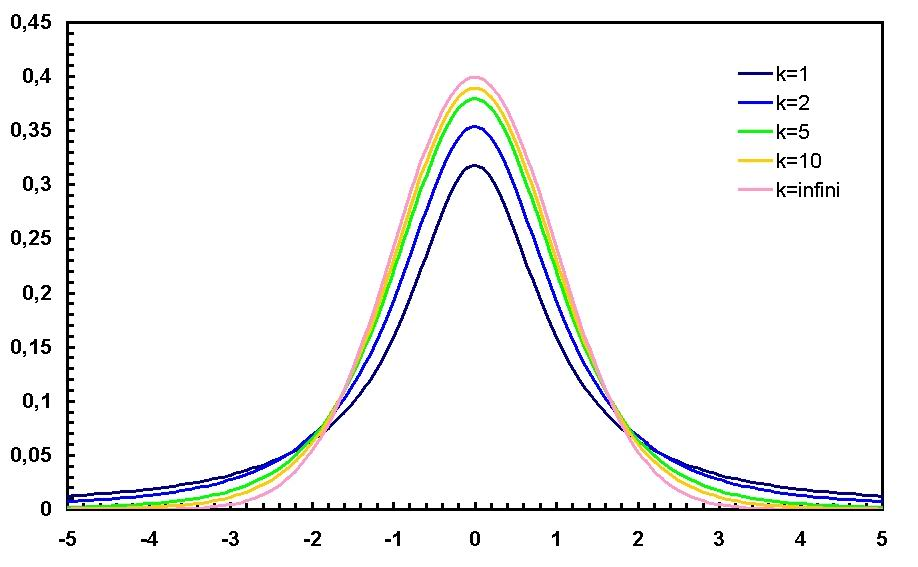
\includegraphics[height=5cm,keepaspectratio=true]{./images/Student_densite_best.jpg}
 % Student_densite_best.jpg: 0x0 pixel, 300dpi, 0.00x0.00 cm, bb=
 \caption{De The original uploader was Thorin de Wikipedia en francés - Transferido desde fr.wikipedia a Commons., CC BY-SA 1.0, https://commons.wikimedia.org/w/index.php?curid=1878902}
 \label{fig:tPDF}
\end{figure}




 \begin{figure}[h]
 \centering
 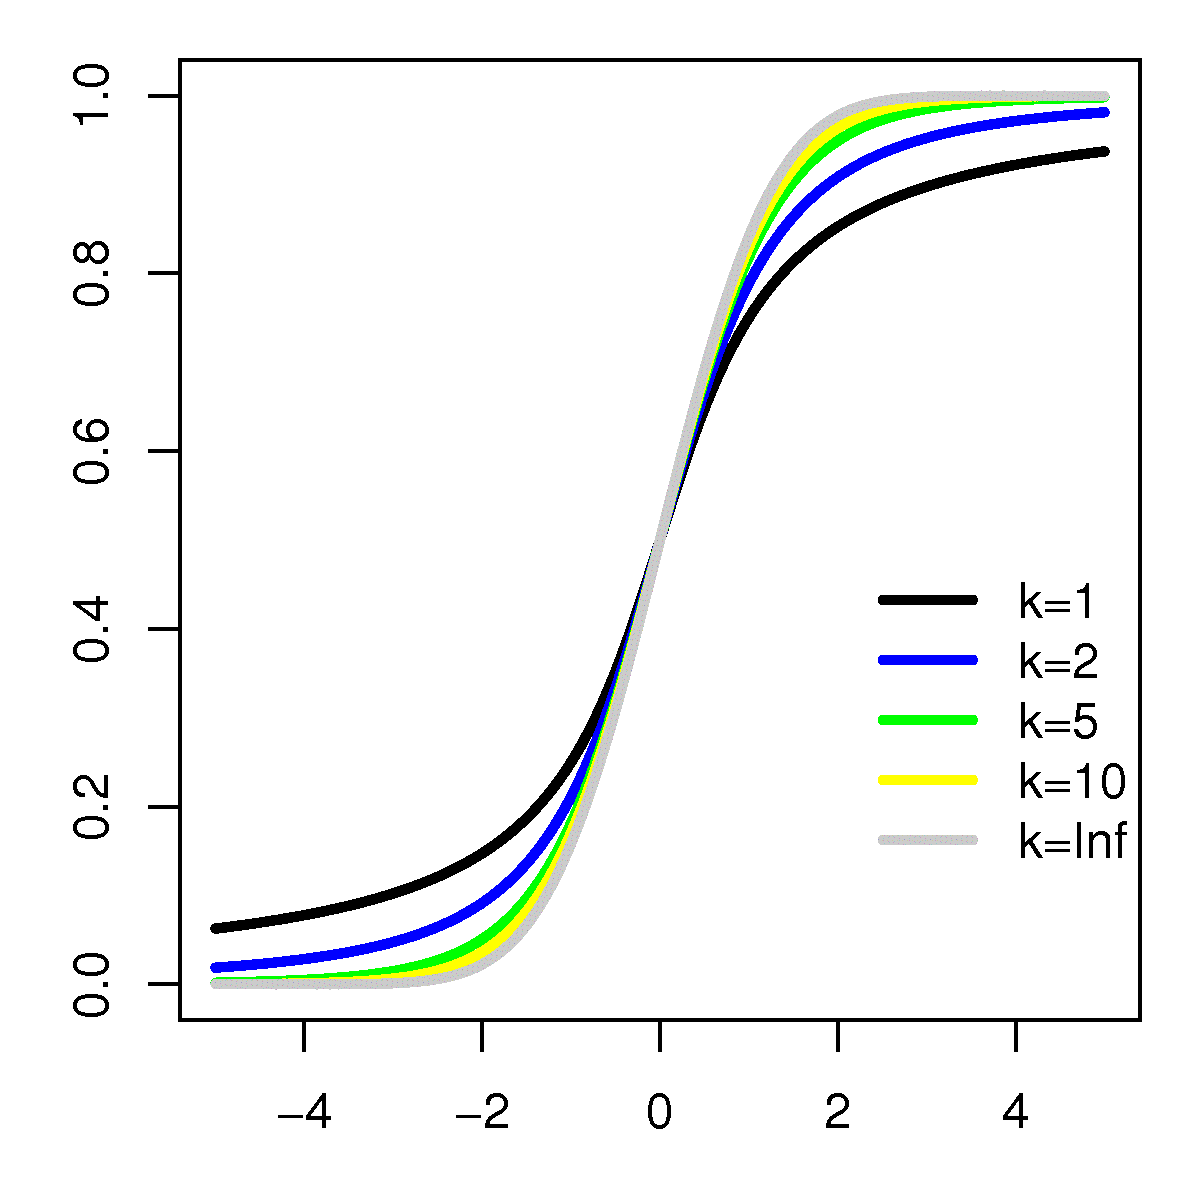
\includegraphics[height=5cm,keepaspectratio=true]{./images/T_distributionCDF.png}
 % T_distributionCDF.png: 0x0 pixel, 300dpi, 0.00x0.00 cm, bb=
 \caption{De Desconocido, CC BY-SA 3.0, https://commons.wikimedia.org/w/index.php?curid=788691}
 \label{fig:tCDF}
\end{figure}

\begin{lstlisting}[language=Python, caption=Distribución $t$ en \texttt{Python}]
from scipy import stats
import numpy as np
import matplotlib.pyplot as plt

def ft(x, nu):
    return stats.t.pdf(x, df=nu)
def Ft(x, nu):
    return stats.t.cdf(x, df=nu)
x = np.arange(-4,4,0.01)
yd = ft(x,30)
yc = Ft(x,30)

fig, ax = plt.subplots()
plt.plot(x, yd, 'r', linewidth=2)
plt.plot(x, yc, 'b', linewidth=2)
plt.ylim(ymin=0)
plt.show()
\end{lstlisting}



\begin{figure}[h]
 \centering
 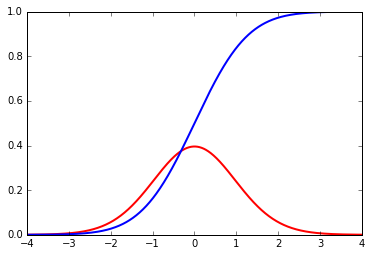
\includegraphics[height=7cm,keepaspectratio=true]{./images/tCDF.png}
 % tPDF.png: 0x0 pixel, 300dpi, 0.00x0.00 cm, bb=
\end{figure}



El parámetro \texttt{df} se le conoce como \emph{grados de libertad} y generalmente se denota como $\nu$ (la letra \texttt{nu} griega).


 Si una variable aleatoria $X$ tiene distribución $t$ con $\nu$ grados de libertad, entonces
 \begin{align}
  \mu_{X}=0, \; \s^{2}_{X}=\dfrac{\nu}{\nu-2}
 \end{align}



 \begin{ejemplo}
  Consideremos una variable con distribución $t$ y $\nu=9$ grados de libertad. Encuentre el valor de $t$ para el cuál el área a la derecha sea $0.05$ pero el total del área sin sombrear sea $0.90$.
  \begin{figure}[h]
 \centering
 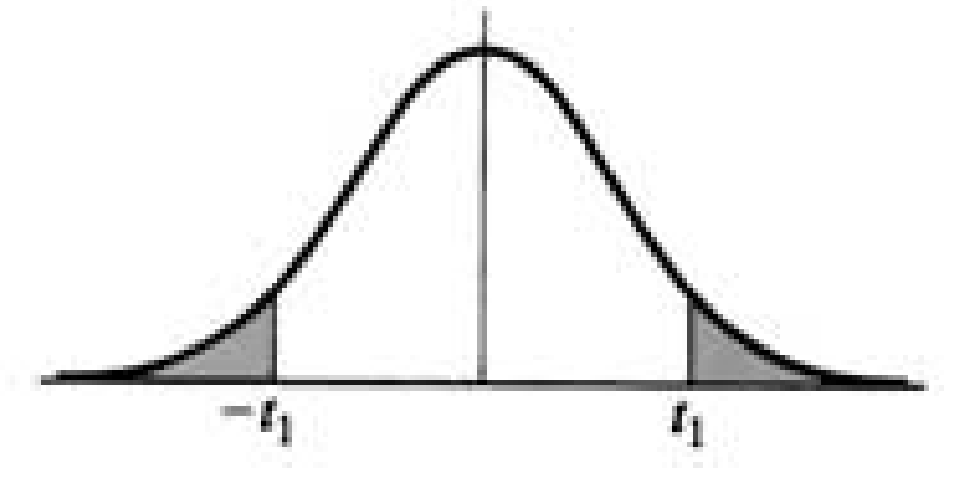
\includegraphics[height=3cm,,keepaspectratio=true]{./images/tExample.png}
 % tExample.png: 0x0 pixel, 300dpi, 0.00x0.00 cm, bb=
\end{figure}

 \end{ejemplo}


[]{tExample.py}
\begin{lstlisting}[language=Python]
from scipy import stats
import numpy as np
import matplotlib.pyplot as plt

def tp(x, nu):
    return stats.t.ppf(x, df=nu)

print tp(0.05, 9)
##-1.83311293265
print tp(1-0.05, 9)
##1.83311293265
\end{lstlisting}

\paragraph{Varianza muestral}
 \begin{align}
  S^{2}=\sum\dfrac{\left( A_{i}-A_{0} \right)^{2}}{n-1}
 \end{align}


\paragraph{Estadístico t}
\begin{align}
 t = \dfrac{\left( A-A_{0} \right)}{S/\sqrt{n}}
\end{align}



\section{Intervalos de confianza, niveles de significación y valores $p$}

\begin{figure}[h]
 \centering
 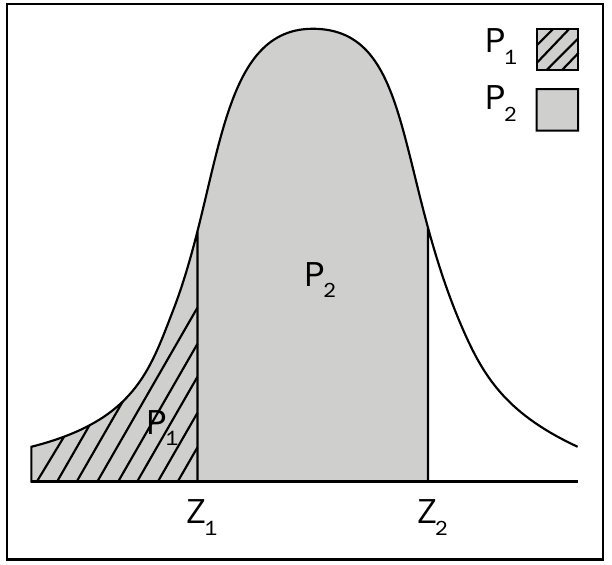
\includegraphics[height=5cm,keepaspectratio=true]{./images/kum0401.png}
 % kum0401.png: 0x0 pixel, 300dpi, 0.00x0.00 cm, bb=
 \caption{Una distribución típica normal con valores $p.$}
 \label{fig:0401}
\end{figure}



Supongamos que $Z_{1}$ y $Z_{2}$ son dos $Z-$estadísticos correspondientes a dos valores de una variable aleatoria y $p_{1}$ y $p_{2}$ son áreas encerradas por la curva de densidad a la derecha de esos valores.

En otras palabras
\begin{align}
 P(X>Z_{1})=p_{1}\\
 P(X>Z_{2})=p_{2}
\end{align}



Entonces, podemos definir un intervalo en el cual encontrar el valor de una variable aleatoria, al cual llamaremos \emph{intervalo de confianza.}


Por ejemplo, para una distribución normal con media $\mu$ y desviación estándar $\sigma,$ el valor de la variable aleatoria estará en el \emph{intervalo} $[\mu-3\s,\mu+3\sigma]$ con una \emph{confianza} (problemaabilidad) del $99\%.$


Para cualquier \emph{estimador} (variable aleatoria) que tenga una distribución normal, uno puede definir un intervalo de confianza si decidimos el nivel de confianza o problemaabilidad.


Podemos pensar en los \emph{intervalos de confianza} cómo el umbral de los valores aceptados para sostener que la \emph{hipótesis nula} es cierta


Si el valor del estimador vive en este rango, será estadísticamente correcto decir que la hipótesis nula es correcta.


Para definir un intervalo de confianza, se necesita definir antes un \emph{nivel (o problemaabilidad) de confianza.}  Esta problemaabilidad necesita ser definida por el investigador dependiendo del contexto.


Digamos que esta problemaabilidad es $p$. En general, utilizaremos el \emph{nivel de significación}
\begin{align}
 \beta = 1-p,
\end{align}
que representa la problemaabilidad de que la hipótesis nula no sea correcta. 

$\beta$ es definida por el investigador y usualmente esta en el orden de $0.01$ a $0.1$.



 Un concepto importante que aprender aquí es el \emph{valor de problemaabilidad} o simplemente \emph{valor-}$p$ de un estadístico:  Es la problemaabilidad de que una variable aleatoria asuma un valor mayor al \emph{valor-}$Z$ (o al \emph{valor-}$t$)
 \begin{align}
  p-\texttt{valor}=P\left( X>Z \right)
 \end{align}



\begin{figure}[h]
 \centering
 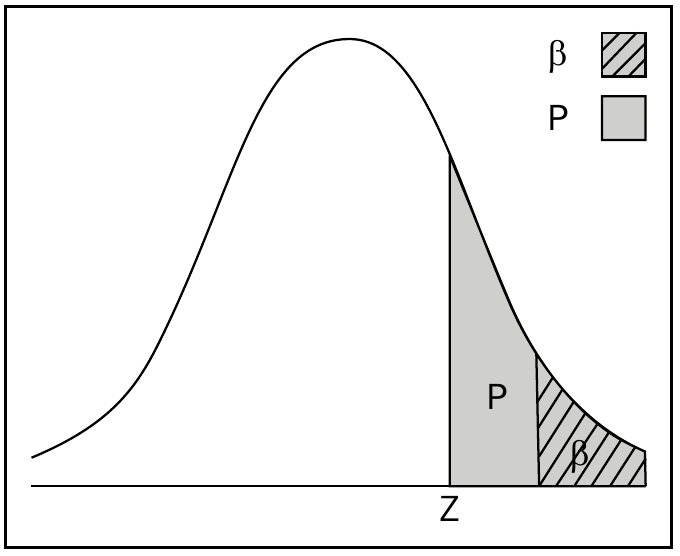
\includegraphics[height=5cm,keepaspectratio=true]{./images/kum0402.png}
 % kum0402.png: 0x0 pixel, 300dpi, 0.00x0.00 cm, bb=
 \caption{Una distribución normal típica con $p-$valores y nivel de significación.}
 \label{fig:0402}
\end{figure}


\paragraph{Criterio}
\begin{itemize}
 \item Aceptar la \emph{hipótesis nula y rechazar la alternativa si $p-\texttt{valor}>\beta$}
 \item Aceptar la \emph{hipótesis alternativa y rechazar la nula si $p-\texttt{valor}<\beta$}
\end{itemize}



Debido a la simetría de la distribución normal, existen tres tipos de pruebas de hipótesis:
\begin{enumerate}
 \item Cola izquierda;
 \item cola derecha;
 \item ambas colas.
\end{enumerate}


\paragraph{Cola izquierda}
\begin{figure}[h]
 \centering
 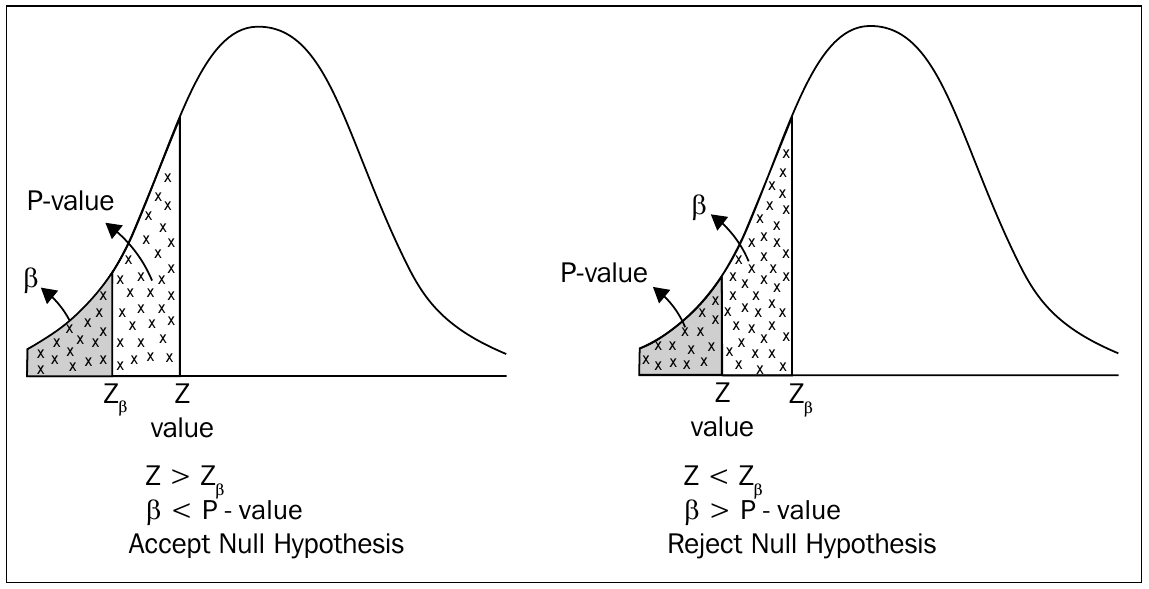
\includegraphics[width=10cm,keepaspectratio=true]{./images/kum0403.png}
 % kum0403.png: 0x0 pixel, 300dpi, 0.00x0.00 cm, bb=
 \caption{Prueba de hipótesis: Cola izquierda}
 \label{kum0403}
\end{figure}


\paragraph{Cola derecha}
\begin{figure}[h]
 \centering
 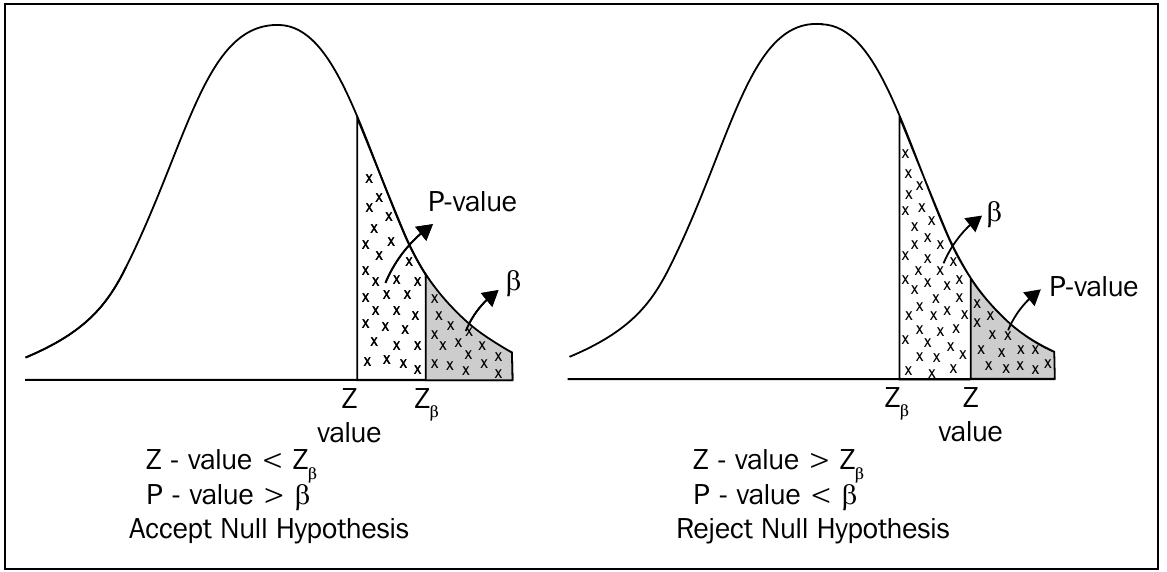
\includegraphics[width=10cm,keepaspectratio=true]{./images/kum0404.png}
 % kum0403.png: 0x0 pixel, 300dpi, 0.00x0.00 cm, bb=
 \caption{Prueba de hipótesis: Cola derecha}
 \label{kum0403}
\end{figure}


\paragraph{Dos colas}
Analizamos ambas colas y si en alguna de las dos colas, falla la respectiva prueba de hipótesis, la prueba de hipótesis se rechaza.


\section{Una guía paso a paso para realizar una prueba de hipótesis}
\paragraph{Paso \#1}
\emph{Defina sus hipótesis nula y alternativa.} Las hipótesis nula es algo que ya se establece y se acepta como cierto, al cuál denotamos como $H_{0}.$ También, suponemos que el valor del parámetro en la hipótesis nula es $A_{0}.$

\paragraph{Paso \#2}
Tome una muestra, digamos de unas 100 o 1000 personas o ocurrencias de eventos, y calcule el valor del estimador (por ejemplo, el promedio del parámetro como es la edad promedio, el tiempo promedio de entrega de la pizza, ingreso promedio, etc.) Digamos que este valor fue $A_{m}.$

\paragraph{Paso \#3}
Calcule el valor normal estándar del valor $Z$
\begin{align}
 Z=\dfrac{A_{m}-A_{0}}{\s/\sqrt{n}}
\end{align}



En la fórmula anterior, $\s$ es la desviación estándar de la población o ocurrencias de eventos y $n$ es el número de personas en la muestra.


La problemaabilidad asociada con el valor $Z$ calculada en el paso $3$ se debe comparar con el nivel de significación de la prueba a determinar si la hipótesis nula será aceptada o rechazada.


\section{Un ejemplo de la prueba de hipótesis}
\paragraph{Planteamiento}
Un famoso restaurante de pizza afirma que su tiempo de entrega es de \emph{20 minutos}, con una desviación estándar de 3 minutos. 

Un investigador de mercados independiente afirma que ellos están desinflando los números para ganar clientes y el tiempo de entrega promedio es de hecho \emph{21.2 minutos}.

¿Es su afirmación justificada o está el negocio de pizza correcto en su afirmación? \emph{Suponga un nivel de significación del $5\%$}


Definamos las hipótesis nula y alternativa:
\begin{itemize}
 \item Lo que el negocio de pizzas afirma: $H_{0}:A_{0}=20.$
 \item Lo que el investigador reclama:
 $H_{a}: A_{0}>20.$
 \item Desviación estándar (conocida): $\s=3.$
 \item Tamaño de la muestra: $n=64.$
 \item Nivel de significación: $\beta=0.05.$
\end{itemize}


Calculemos el valor $Z$:
\begin{align}
 Z=\dfrac{21.2-20}{3/\sqrt{64}}=3.2
\end{align}



Denotemos por $F$ la función de distribución acumulativa de una variable normal $N(0,1).$ 

Calculamos el valor $p$ correspondiente al valor $Z=3.2$:
\begin{align}
 \texttt{valor-p}&=1 - F(3.2)\\
 &=1-0.999312862062\\
 &= 0.000687137937916
\end{align}



 Esto significa que si la media fuera $A_{0}=20,$ la problemaabilidad de que la media muestral fuera $A=21.2$ es $\approx 0.069\%.$
 

 Como \emph{elegimos} un nivel de significación $\beta=5\%,$ y $0.069\% < 5\%,$ podemos rechazar la hipótesis nula $H_{0}: A_{0}=20.$


\begin{figure}[h]
 \centering
 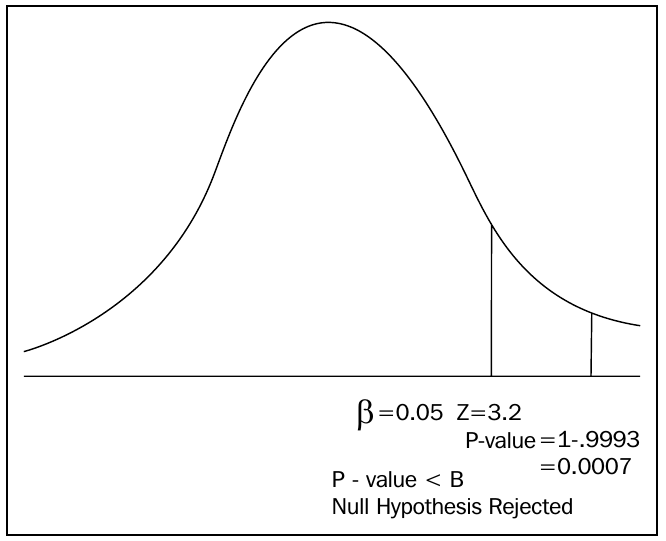
\includegraphics[height=5cm,keepaspectratio=true]{./images/kum0405.png}
 % kum0405.png: 0x0 pixel, 300dpi, 0.00x0.00 cm, bb=
 \caption{La hipótesis nula se rechaza porque el $p-$valor es menor al nivel de significación $\beta$.}
 \label{fig:0405}
\end{figure}


\section{Prueba $\chi-$cuadrada}

La \emph{prueba $\chi^{2}$} se usa comúnmente para comparar \emph{datos observados vs datos esperados} suponiendo que los datos siguen ciertas hipótesis.


Debemos suponer cierta hipótesis, la cuál nuestros datos seguirán y calculamos los datos esperados de acuerdo a esa hipótesis.


Debemos ya tener los datos observados, y calcular la desviación entre estos y los esperados usando el estadístico definido en la siguiente fórmula:
\begin{align}
 \texttt{valor }\chi^{2}\texttt{:} g= \sum\dfrac{\left( O-E \right)^{2}}{E},
\end{align}
donde $O$ es el valor observado y $E$ el esperado, con la suma sobre todos los posibles datos.

\paragraph{Aplicaciones del estadístico $\chi-$cuadrada}
La prueba de ji cuadrado se puede usar para hacer lo siguiente:
\begin{itemize}
\item Mostrar una relación causal o independencia entre una variable de entrada y otra de salida.  
\item Verificar si los datos observados provienen de una fuente justa / imparcial. 
\item Comproblemaar si los datos son demasiado buenos para ser verdad.
\end{itemize}


\paragraph{Ejemplo}
Realicemos un experimento hipotético en el que una moneda se lanza 10 veces. ¿Cuántas veces espera obtener ya sea un águila o un sol?  La respuesta adecuada sería 5.  Ahora bien, ¿qué pasaría si realizamos este experimento 1000 veces y registramos los números de águilas y soles.


Supongamos que observamos soles 553 veces y águilas el resto de ocasiones:
\begin{center}
 $H_{0}:$ La proporción de soles y águilas es $0.5$ \\
 $H_{a}:$ La proporción no es $0.5$
\end{center}



\begin{center}
\begin{tabular}{|l|l|l|}\hline
 & Soles & Águilas\\\hline
Observado & 553 & 447\\\hline
Esperado & 500 & 500\\\hline
\end{tabular}
\end{center}


Calculemos el valor $\chi^{2}:$
\begin{align}
 g = \dfrac{\left( \left( 553-500 \right)^{2}+\left( 447-500 \right)^{5} \right)}{500}\approx 11.236
\end{align}



Este valor$-\chi^{2}$ se compara al valor en una \emph{distribución $\chi^{2}$} para un número dado de \emph{grados de libertad} y un nivel de significación.

\paragraph{La Distribución $\chi^{2}$}
Sean $X_{1},X_{2},...,X_{\nu}$ variables aleatorias independientes $N(0,1).$
 Consideremos la variable aleatoria
\begin{align}
 \label{outline:19}
 \chi^{2}=X_{1}^{2}+...+X_{\nu}^{2}
\end{align}
a la que llamaremos \emph{chi cuadrada.} Su correspondiente distribución de problemaabilidad recibe el mismo nombre.

\paragraph{Propiedades de $\chi^{2}$}
\begin{align}
 \label{eq:22}
 \mu=\nu, \; \s = 2\nu
\end{align}


[]{scipy.stats.chi2}
\begin{lstlisting}[language=Python]
from scipy.stats import chi2
import numpy as np
import matplotlib.pyplot as plt
fig, ax = plt.subplots(1, 1)

df = 55

x = np.linspace(chi2.ppf(0.01, df),
 chi2.ppf(0.99, df), 100)
ax.plot(x, chi2.pdf(x, df),'r-',
 lw=5, alpha=0.6, label='chi2 pdf')
\end{lstlisting}



\begin{figure}[h]
 \centering
 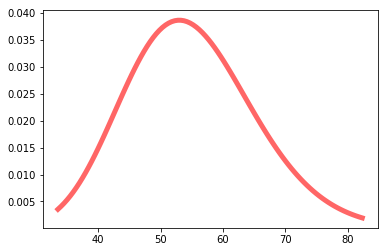
\includegraphics[height=5cm,keepaspectratio=true]{./images/statsChi2.png}
 % statsChi2.png: 0x0 pixel, 300dpi, 0.00x0.00 cm, bb=
 \caption{Función de densidad de distribución $\chi^2$ con $\nu=55$}
 \label{fig:Chi2}
\end{figure}


[]{\texttt{statsChi2.py}}
\begin{lstlisting}[language=Python]
from scipy.stats import chi2
import numpy as np
import seaborn as sns
import matplotlib.pyplot as plt

sns.set_palette("husl")
fig, ax = plt.subplots(1, 1)

for df in range(2,15+1):
    x = np.linspace(chi2.ppf(0.01, df),
                    chi2.ppf(0.99, df), 100)
    ax.plot(x, chi2.pdf(x, df), label='chi2 pdf')
\end{lstlisting}



\begin{center}
 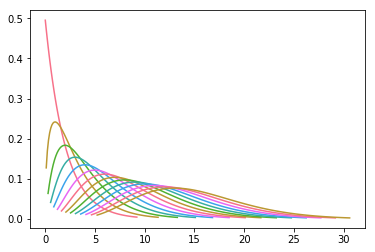
\includegraphics[height=7cm,keepaspectratio=true]{./images/statsChi2Several.png}
 % statsChi2Several.png: 0x0 pixel, 300dpi, 0.00x0.00 cm, bb=
\end{center}


\paragraph{Regresando a nuestro ejemplo...}
El número de grados de libertad es el número de categorías menos uno.  En nuestro ejemplo $\nu = 2-1 =1.$  Supongamos un nivel de significación $\beta=0.05.$


\begin{figure}[h]
 \centering
 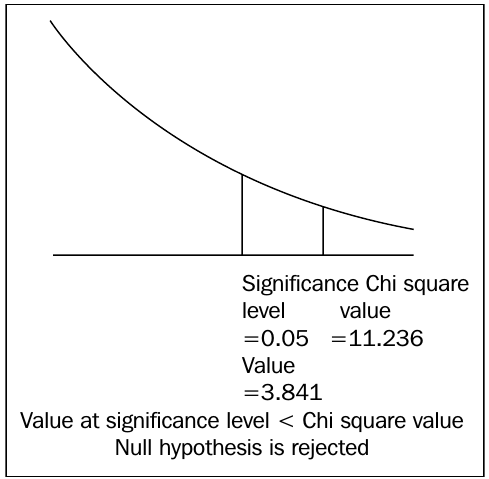
\includegraphics[height=5cm,keepaspectratio=true]{./images/kum0407.png}
 % kum0407.png: 0x0 pixel, 300dpi, 0.00x0.00 cm, bb=
 \caption{La hipótesis nula se rechaza porque el valor del estadístico $\chi^2$ al nivel de significación es menor que el valor del estadístico.}
 \label{fig:0407}
\end{figure}


[]{Otro ejemplo}
Examinemos otros ejemplo donde queremos demostrar que el género de un estudiante y las materias que escoge son independientes.


Supongamos que un grupo de estudiantes, la siguiente tabla representa el número de hombres y mujeres que toman matemáticas, arte y comercio como sus materias principales.


\begin{center}
\begin{tabular}{|l|l|l|l|l|}\hline
 & Matemáticas & Artes & Comercio & Total\\\hline
Hombres & 68 & 52 & 90 & 210\\\hline
Mujeres & 28 & 37 & 35 & 100\\\hline
Total & 106 & 89 & 125 & 310\\\hline
\end{tabular}
\end{center}



Si en la elección de las materias, no fuera relevante el género, entonces el número esperado de hombres y mujeres tomando diferentes materias sería
\begin{center}
\begin{tabular}{|l|l|l|l|l|}\hline
 & Matemáticas & Arte & Comercio & Total\\\hline
Niños &  &  &  & \\\hline
Niñas &  &  &  & \\\hline
Total &  &  &  & \\\hline
\end{tabular}
\end{center}



Las desviaciones se calculan usando la fórmula
$(O-E)^2/E$:
\begin{center}
\begin{tabular}{|l|l|l|l|l|}\hline
 & Matemáticas & Arte & Comercio & Total\\\hline
Hombres &  &  &  & \\\hline
Mujeres &  &  &  & \\\hline
Total &  &  &  & \\\hline
\end{tabular}
\end{center}

El estadístico $\chi^{2}$ se obtiene al sumar todos estos valores.

\paragraph{Conclusiones (del profesor)}
Como $\chi^{2}= 4.99$ y el valor del estadístico $\chi^{2}$ a un nivel se significación es $11.07,$ la hipótesis nula se acepta.

De manera equivalente
\begin{align}
 \texttt{valor-}p=1- F_{\chi^{2}}(4.99)=0.416991040312>\beta=0.05,
\end{align}
 obtenemos la misma conclusión:
 \begin{center}
  \emph{La elección de materias es independiente del género.}
 \end{center}


